\section{Results}

\newcommand{\takeaway}[1]{
\vspace{6pt}
\noindent\fbox{\parbox{\columnwidth}{#1}}
\vspace{6pt}
}

\mike{Results and Discussion:}
\begin{itemize}
    \item (Overview) Give an overview of results, possibly referencing a graph or two.
    \item Statistical analysis: provide positive and null hypotheses for the research questions.
    \item Evaluation of research questions: statistical results and explanations of the graphs.  One subsection per research question?
    \item Threats to validity: what are our threats?
    Internal validity: not really necessary, I think.
    External validity (how much can the results be generalized):
        1. currently all models are *very small*;
        2. Many programs were drawn from mutations of a relatively small number of ``seed'' programs;
        3. The models are written in Lustre rather than FOL.  This means that the
            top-level conjunctions are all over equations rather than general
            form;
        4. Others?!?
    Construct validity: we are measuring what we think we're measuring: IVC and minimality are reasonably defined.  For discussions of ``completeness'' and ``traceability'' we need to be clear about any claims (probably not in this paper).
\end{itemize}

\subsection{Performance}
\label{sec:performance}

In this subsection, we examine the performance of our inductive validity core algorithms (research question \textbf{RQ1}).  First we examine the performance overhead of the IVC algorithm over the time necessary to find a proof using inductive model checking.  To examine this question, we use the default {\em fastest} option of JKind which terminates when either the k-induction or PDR algorithm finds a proof.  To measure the performance overhead of the \ucalg\ algorithm, we execute it over the proof generated by the {\em fastest} option.

Since the \ucalg\ algorithm uses the UNSAT-core facilities of the underlying SMT solver, the performance is dependent on the efficiency of this part of the solver.  Examining Table~\ref{tab:overhead}, it is possible to examine both the aggregate computation time for analysis using the four solvers under evaluation and the overhead imposed by the \ucalg\ algorithm.  The data suggests that Z3 is the most performant solver both in terms of computation time and overhead.  Figure~\ref{fig:runtimez3} allows a visualization of the overhead for the Z3 solver, where the models are ranked on the x axis in terms of their analysis time without performing \ucalg, and the y-axis describes analysis time with and without \ucalg.

\mike{Add the raw timings for each solver for proof and proof + \ucalg\ analysis in Table~\ref{tab:overhead}.}

Although it is relatively obvious from Table~\ref{tab:overhead}, it is straightforward to demonstrate with statistical significance that Z3 outperforms other solvers.  The hypotheses are as follows: \mike{FILL IN HYPOTHESES}.

\takeaway{The IVC algorithm with the Z3 SMT solver adds a modest and reasonably stable performance penalty to inductive proofs.}

Next, we consider the overhead of \ucalg\ vs. \bfalg.  Recall from Section~\ref{sec:ivc} that \bfalg\ requires $n$ model checking runs, where $n$ is the number of conjuncts in the transition relation. As expected, the performance is approximately a linear multiple of the size of the model, so larger models yield substantially lower performance.\footnote{for Lustre models, the number of conjuncts is equivalent to the number of equations in the Lustre model.}  We run the brute-force algorithm using Z3 as it is the most performant (on average) of the solvers.  For \mike{YYY} models, \bfalg\ times out after 1 hour.   Figure~\ref{fig:runtimeall} presents the overhead of {\em all} \ucalg\  solutions from different solvers as compared to the overhead of the brute-force algorithm.

\takeaway{The brute-force algorithm \bfalg\ adds a substantial performance penalty to inductive proofs in all cases and is not scalable enough to compute a minimal core for large analysis problems.}

\begin{table}
  \centering
  \begin{tabular}{ |c||c|c|c|c| }
    \hline
     solver & min & max & mean & stdev \\[0.5ex]
    \hline
    Z3   & 0.726\% & 45.396\% & 13.414\% & 11.369\% \\[0.5ex]
    Yices &   0.200\%  & 262.254\%   & 47.264\% & 51.193\% \\[0.5ex]
    SMTInterpol& 0.930\% & 268.571\% &  70.500\% & 58.541\%\\[0.5ex]
    MathSAT & 0.502\% & 396.124\% &  71.007\% & 79.990\%\\[0.5ex]
    \hline
  \end{tabular}
  \caption{Overhead of \ucalg\ computations using different solvers}
  \label{tab:overhead}
\end{table}

\mike{Integrate these two aspects better}

\textbf{Timing analysis.} Table~\ref{tab:eff-comp-jsup} compares overall runtime of support computation in different solvers and \texttt{JSupport}, which helps to see if any solvers outperform others in terms of performance.
\ela{will add hypotheses}
\begin{table}
  \centering
  \begin{tabular}{ |c||c|c|c|c| }
    \hline
     runtime (sec) & min & max & mean & stdev \\[0.5ex]
    \hline\hline
    JSupport & 2.381 & 165.157 & 21.533 & 23.533 \\[0.5ex]
    Z3   & 0.112 & 42.928 & 2.412 & 5.009 \\[0.5ex]
    Yices &   0.111  & 39.657   & 2.464 & 5.224 \\[0.5ex]
    SMTInterpol& 0.225 & 514.886 &  4.331 & 26.411 \\[0.5ex]
    MathSAT & 0.111 & 43.623 &  2.765 & 5.157 \\[0.5ex]
    \hline
  \end{tabular}
  \caption{\small{\texttt{ReduceSupport} runtime with different solvers compared to \texttt{JSupport}}}
  \label{tab:eff-comp-jsup}
\end{table}

\mike{This section will have be rewritten}
\textbf{RQ5.} The size of the models in our benchmark is between 0 KB and 10 KB.
We divided the models into 9 different categories based on their size such that $category_i$ contains
all models whose sizes are between $(i - 1)$ KB and $i$ KB. Then, using Definition~\ref{def:dis}, distance for each model in each category was calculated. After that, minimum, maximum, average, standard deviation of the data were obtained per category. To analyze data, we use hypothesis testing; since in RQ4, we calculated average of $D_{J\{M\}}$ among all models, we consider it as population mean and formulate the following hypotheses:
\begin{itemize}
  \item H0: given $category_i$,
  \begin{itemize}
    \item if $i < 5$, mean of $D_{J\{M\}}$ in $i$ is less than population mean of $D_{J\{M\}}$
    \item if $i \geq 5$, mean of $D_{J\{M\}}$ in $i$ is greater than population mean of $D_{J\{M\}}$
  \end{itemize}
  \item H1: given $category_i$, average $D_{J\{M\}}$ in $i$ could be less or
  greater than equal to the population mean.
\end{itemize}

Table~\ref{tab:modelsize} summarizes the result of this analysis; the column \emph{n} in the table shows the number of models in each category (sample size), which means the sum of the numbers in the column is 405 (for example, there are 6 models whose sizes are between 8 KB and 9 KB, and in all of them \textit{similarity} is 1.0).


\begin{table}
  \centering
  \begin{tabular}{ |c|c|c|c|c|c|c|c|}
    \hline
    size (KB) & n&
     min & max & mean & stdev & ES & p-value \\[0.5ex]
    \hline\hline
    % For p-value:
    % mean_H0 = 0.096  std = 0.132 ---- obtained from RQ4
    % t = (mean − mean_H0)/(stdev/sqrt(sample_size))
    [0-1] & 49 & 0.0 & 0.333 & 0.084 & 0.131 & 0.09 & < 0.2626 \\[0.5ex] % t = -0.64
    [1-2] & 90& 0.0 & 0.667 & 0.139 & 0.157 & 0.33 & < 0.00548 \\[0.5ex] % t= 2.598
    [2-3] & 26&0.0 & 0.5 & 0.124 & 0.132 & 0.21 & < 0.1452 \\[0.5ex] % t = 1.08
    [3-4] & 34&0.0 & 0.333 & 0.076 & 0.124 & 0.15 & < 0.1770\\[0.5ex] % t = -0.94
    [4-5] & 88&0.0 & 0.879 & 0.090 & 0.134 & 0.05 & < 0.3377\\[0.5ex] % t = 0.4200
    [5-6] & 11&0.0 & 0.25 & 0.170 & 0.107 & 0.56 & < 0.0225\\[0.5ex] % t = 2.2937
    [6-7] & 2&0.0 & 0.042 & 0.021 & 0.021 & 0.57 & < 0.0622\\[0.5ex] % t = -5.051
    [7-8] & 99&0.0 & 0.398 & 0.067 & 0.094 & 0.22 & < 0.00138\\[0.5ex]% t = 3.069
    [8-9] & 6&0.0 & 0.0 & 0.0 & 0.0 & 0.72 & < 0.00001\\[0.5ex] %t = inf
    \hline
  \end{tabular}
  \caption{Model size vs similarity among its support sets}\label{tab:modelsize}
\end{table}

\vspace{6pt}
\noindent\fbox{%
    \parbox{\columnwidth}{%
     The size of the model does not affect the stability of our algorithm;
     if a model is large, it does not necessarily mean that it will have a lot of different minimal support sets.
    }%
}
 \vspace{6pt}



\begin{figure}
  \centering
  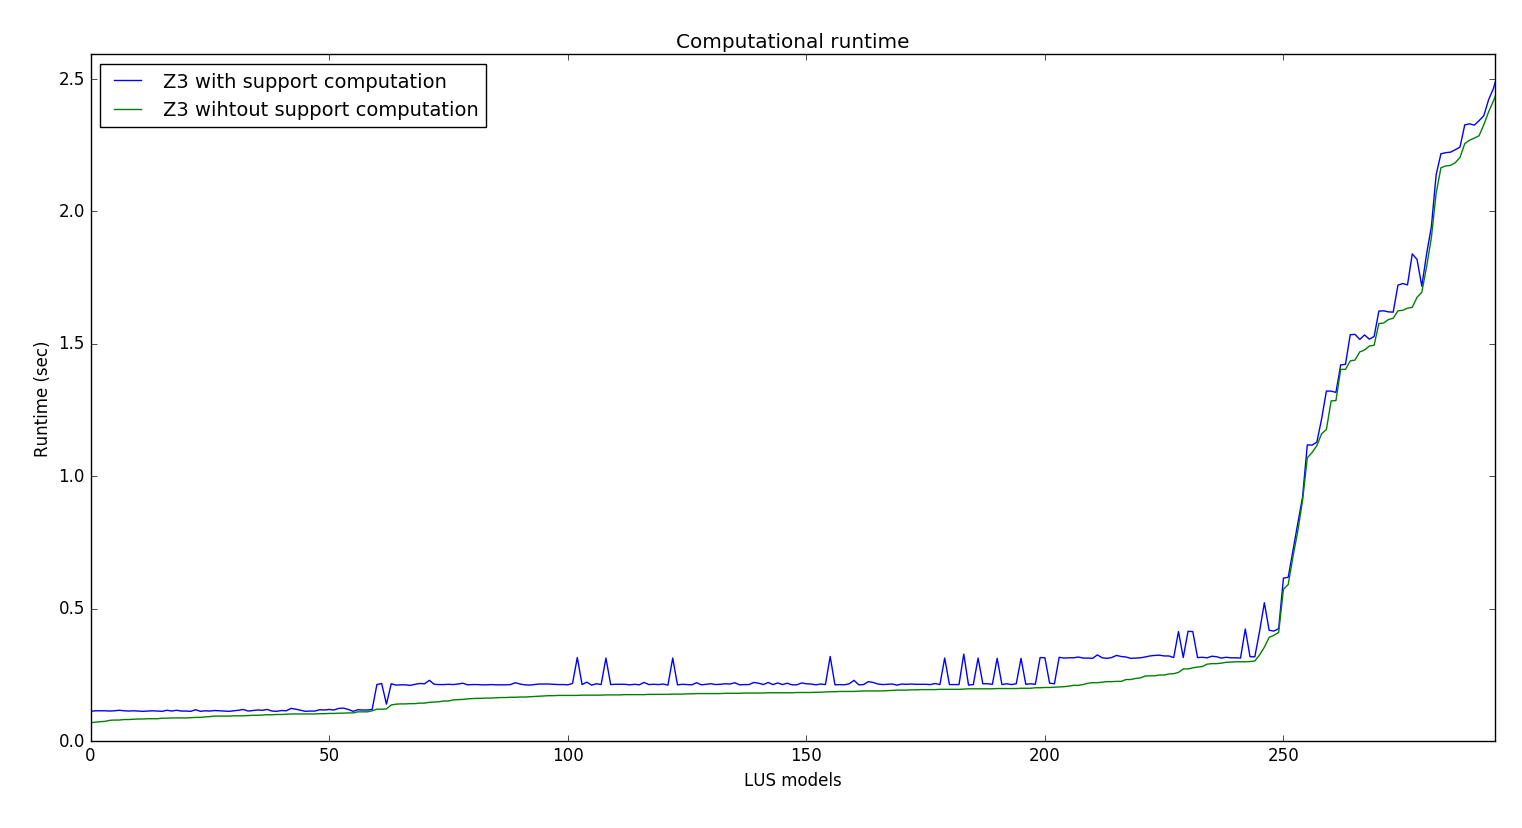
\includegraphics[width=\columnwidth]{figs/runtimeZ3.png}
  \mike{I do not think this figure is necessary}
  \caption{Runtime of \texttt{JKind} with/without support computation}\label{fig:runtimez3}
\end{figure}


\begin{figure}
  \centering
  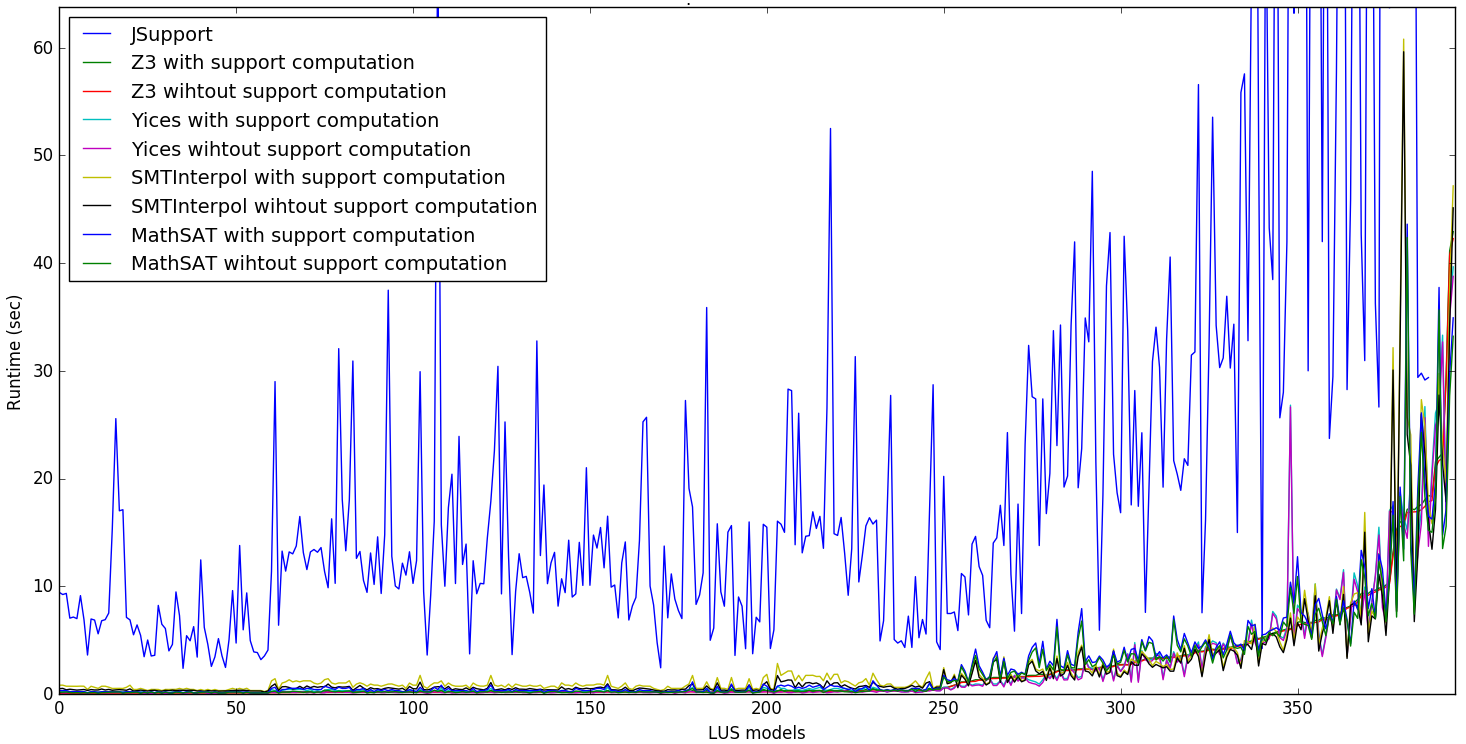
\includegraphics[width=\columnwidth]{figs/runtimeAll.png}
  \mike{There is a spelling error in the key.  Also, what the ordering in this figure?
  Is it z3 running without IVC?}
  \caption{Runtime of \ucalg\ computation with all solvers compared to \bfalg\ algorithm in Z3}\label{fig:runtimeall}
\end{figure}

\begin{table}
  \centering
  \begin{tabular}{ |c|c|c| }
    \hline
     brute-force & PDR & k-induction \\
    \hline
      1 & 2 & 3  \\
    \hline
  \end{tabular}
  \caption{Minimality of IVC computation using different algorithms}
  \label{tab:minimality-algorithm}
\end{table}

\begin{table}
  \centering
  \begin{tabular}{ |c|c|c| }
    \hline
     solver & aggregate & \% increase over minimal \\
    \hline
    brute-force & 3078 & * \\
    z3 & ?? & XX\% \\
    yices & ?? & YY\% \\
    MathSAT & ?? & ZZ\% \\
    SMTInterpol & ?? & AA\% \\
    \hline
  \end{tabular}
  \caption{Minimality of IVC computation using different solvers}
  \label{tab:minimality-solver}
\end{table}

\begin{figure}
  \centering
  \mike{Placeholder for figure here!}
  \mike{Placeholder for figure here!}
  \mike{Placeholder for figure here!}
  \mike{Placeholder for figure here!}
  \mike{Placeholder for figure here!}
  \mike{Placeholder for figure here!}
  \mike{Placeholder for figure here!}
  \caption{Minimality of cores produced by \ucalg\ algorithm from multiple solvers compared to \bfalg\ algorithm with Z3}
  \label{fig:minimality-all}
\end{figure}

\subsection{Minimality}
\label{sec:minimality}
In this section, we examine the minimality of the cores computed by the \ucalg\ algorithm using different inductive proof methods and compare it to the cores produced by the brute-force algorithm (\textbf{RQ2}).  There are two interesting aspects to be examined related to this research question.  First (\textbf{RQ2.1}), does the choice of algorithm used to produce a proof (k-induction or PDR) matter in terms of the minimality of the inductive core?   As mentioned in Section~\ref{sec:ivc}, the \ucalg\ algorithm is not guaranteed to produce a minimal core due to the role of invariants used in producing a proof; as k-induction and PDR use different invariant generation algorithms, it is possible that one or the other is more likely to yield smaller invariant sets.  In addition, as discussed in Section~\ref{sec:experiment}, k-induction is unable to solve all of the analysis problems; therefore we include only models that are solvable using both k-induction and PDR.  Examining the aggregate data in Table~\ref{tab:minimality-algorithm}, if we sum all elements of all cores together, that PDR has an smaller core size in aggregate than k-induction.  However, the data is noisy, and to examine \textbf{RQ2.1} systematically, we construct a hypothesis that PDR will, in general, equal or outperform k-induction on an arbitrary model:

\mike{ADD HYPOTHESIS/NULL HYPOTHESIS HERE}

Although the aggregate data suggests that PDR will yield a smaller core (on average) than k-induction, this claim is not supported for a given model with significance.

\takeaway{Neither PDR nor k-induction is yields a smaller inductive validity core with statistical significance.}

The second relevant question (\textbf{RQ2.2}) asks how close to minimal are the cores produced by \ucalg\ vs. the (guaranteed minimal) cores produced by the \bfalg\ algorithm?  Note that we cannot measure the distance on all models because the brute-force algorithm times out on many of the larger models.  We therefore examine the distance from minimal cores produced by the brute force algorithm for models in which it completes within the one hour timeout.  For comparison, we run the \ucalg\ algorithm in each tool with the default {\em fastest} algorithm, which will use the result of either k-induction or PDR.  The aggregate results are shown in Table~\ref{tab:minimality-solver}, and a graph showing the performance on each model, ranked along the x-axis by the size of the core produced by \bfalg\ is shown in Figure~\ref{fig:minimality-all}.  The figure demonstrates that while on average there is a modest change in minimality that there can be substantial variance on the sizes of the cores produced by the \ucalg\ algorithm.  This is in part due to {\em diversity} of minimal cores, which is the subect of Section~\ref{sec:diversity}.

\takeaway{The \ucalg\ algorithm computes cores that are XX\% to YY\% larger than those produced by \bfalg, with substantial variance in the results.}

\mike{Should we mention post-processing the \ucalg\ core to find a minimal core using \bfalg?  This might have acceptable performance and guaranteed minimal cores.}
%Because of this variance, in future work, we will extend  post-processing brute-force phase in which we

\iffalse
\ela{I think this is not needed: \\In terms of size, we calculated the size of the biggest and smallest sets per model, then added them together for all models. The same calculation has been done for \texttt{JSupport}:
\begin{itemize}
  \item $A\_JS$: the aggregate number of elements in support sets computed by \texttt{JSupport} = 3078
  \item $A\_Ss$: the aggregate number of elements in the \emph{smallest} support sets = 3474;
  this implies $A\_Ss$ is 12\% greater than $A\_JS$.
  \item $A\_Bs$: the aggregate number of elements in the \emph{biggest} support sets = 3586;
  this implies $A\_Bs$ is 16\% greater than $A\_JS$.
\end{itemize}}
Average size of sets computed by \texttt{ReduceSupport} is 8.55. And, average size of sets computed by \texttt{JSupport} is 7.60. Therefore, in average, support sets computed by \texttt{ReduceSupport} are 88\% close to minimal, in terms of their size.  %  (1 - ((8.55 - 7.6)/ 7.6))  * 100 = 87.5%
Since \texttt{JSupport}, with a great percentage, most of the time computed the smallest support set, we compared the size of the sets computed by \texttt{ReduceSupport} with \texttt{JSupport}. For each configuration, we collected the difference between its support size and \texttt{JSupport} per model. Table~\ref{tab:minimality} shows the result of analysis.
\fi

\subsection{Diversity}
\label{sec:diversity}
Recall from Section~\ref{sec:ivc} that a {\em minimal} core is any core leading to a proof such that if you remove any of the conjuncts from the core, it no longer produces a proof.  For certain models and properties, it is possible that there are many minimal cores that will lead to a proof.  In this section, we examine the issue of diversity: do different tools and algorithms lead to {\em different} minimal cores?  This is both a function of the models and the solution algorithms: for certain models, there is only one possible minimal core, whereas other models might have many. Given that there are multiple solutions, the interesting question is whether using different tools and algorithms will lead to different solutions.  Note that this question is closely tied to that of {\em minimality}, which we examined in the previous section.

Our exploration is not exhaustive, but only exploratory.  The reason that we consider it is that it has substantial relevance to some of the uses of the tool: e.g., for constructing traceability matrices from proofs.  Given diversity of results, we may wish to distinguish {\em must} traceability elements from {\em may} traceability elements across a set of diverse solutions, and consider more systematic explorations of diversity in future work.

To measure diversity of IVCs, we use Jaccard distance~\mike{citation?}:
\begin{definition}{\emph{Jaccard distance:}}
  \label{def:dj}
  $d_J(\small{A}, \small{B}) = 1 - \frac{|A \cap B|}{|A \cup B|} ,\\ 0 \leq d_J(\small{A}, \small{B}) \leq 1$
\end{definition}
\noindent Jaccard distance is a standard metric for comparing finite sets (assuming that both sets are non-empty) by comparing the size of the intersection of two sets over its union.  For each model in the benchmark, the experiments generated 13 different sets of support. Therefore, we obtained $\binom{13}{2} = 78$ combinations of pairwise distances per model. Then, minimum, maximum, average, and standard deviation of the distances were calculated (Fig~\ref{fig:jacdis}), by which, again, we calculated these four measures among all 405 models.  As seen in Table~\ref{tab:78com}, on average, the Jaccard distance between different solutions is small, but the maximum is close to 1, which indicates that even for our exploratory analysis, there are models for which the tools yield substantially diverse solutions.

%The following hypotheses are used to evaluate the results shown in Table~\ref{tab:78com}:
%\begin{itemize}
%  \item H0: there are pairwise configurations that generate very different support sets (with an average Jaccard distance of 0.2)
%  \item H1: each pair of configurations generates very similar support sets (with an average Jaccard distance less than 0.2)
%\end{itemize}

\begin{table}
  \centering
  \begin{tabular}{ |c|c|c|c|c|c| }
    \hline
     min & max & mean & stdev & ES & p-value\\[0.5ex]
    \hline
    %sample size = 4196
     0.0   & 0.882 & 0.027 & 0.062 & 2.79 & < 0.00001 \\[0.5ex]
    \hline
  \end{tabular}
  \caption{Pairwise Jaccard distances among all models}
  \label{tab:78com}
\end{table}

%summarizes the result of this analysis:
%\begin{itemize}
%  \item minimum Jaccard distance among all models is: 0.0
%  \item maximum Jaccard distance among all models is: 0.882
%  \item average Jaccard distance among all models is: 0.027
%  \item standard deviation of Jaccard distance among all models is: 0.062
%\end{itemize}

\begin{figure}
  \centering
  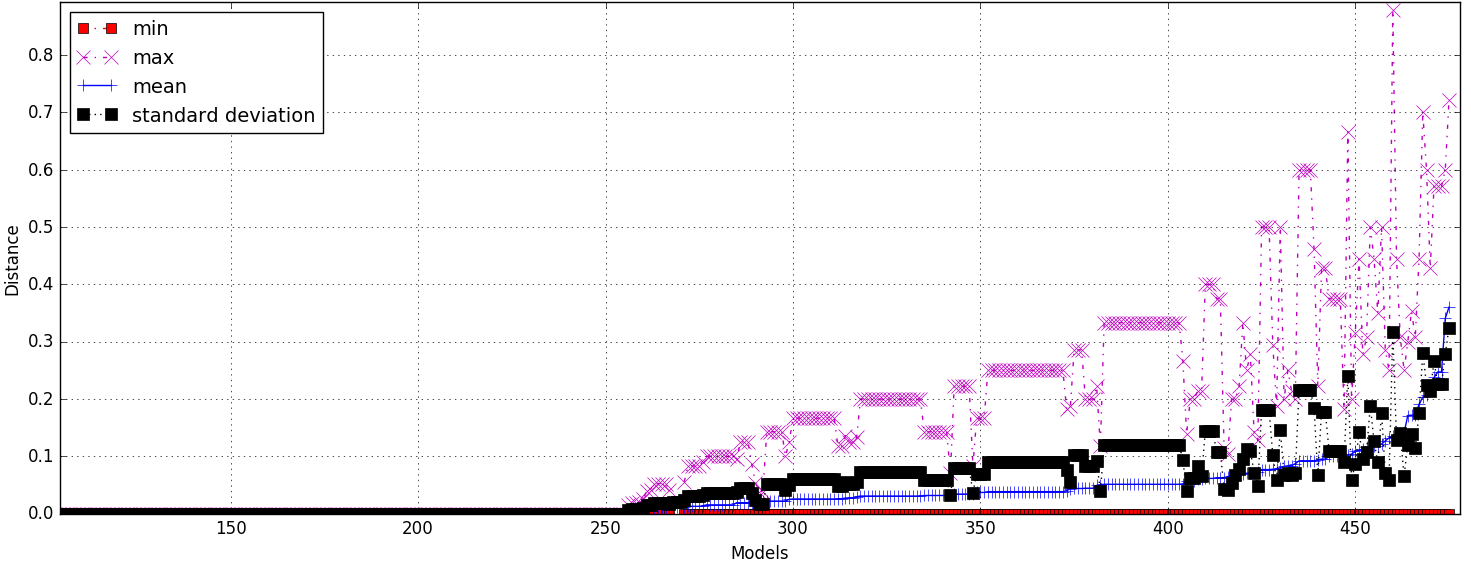
\includegraphics[width=\columnwidth]{figs/jacdis2.png}
  \caption{Pairwise Jaccard distance between support sets}\label{fig:jacdis}
\end{figure}


%\textbf{(3)}  Fig~\ref{fig:maxdis} and Fig~\ref{fig:mindis} shows the results. As you can see, different configurations of \texttt{JKind} do not affect very much the variety of the generated sets. However, \texttt{JSupport} and \texttt{JKind} configurations have had maximum distances most of the time. Even so, the frequency of such maximum distances among 405 models is very low. Table~\ref{tab:pairminmax} shows the percentage that two configurations has the maximum Jaccard distance
%\ela{this is a misleading approach because maximum jaccard distance doesn't mean a big jaccard distance. for this reason, I remove it. related results for this section is in file support_variety_analyses.txt }

%\begin{figure}
%  \centering
%  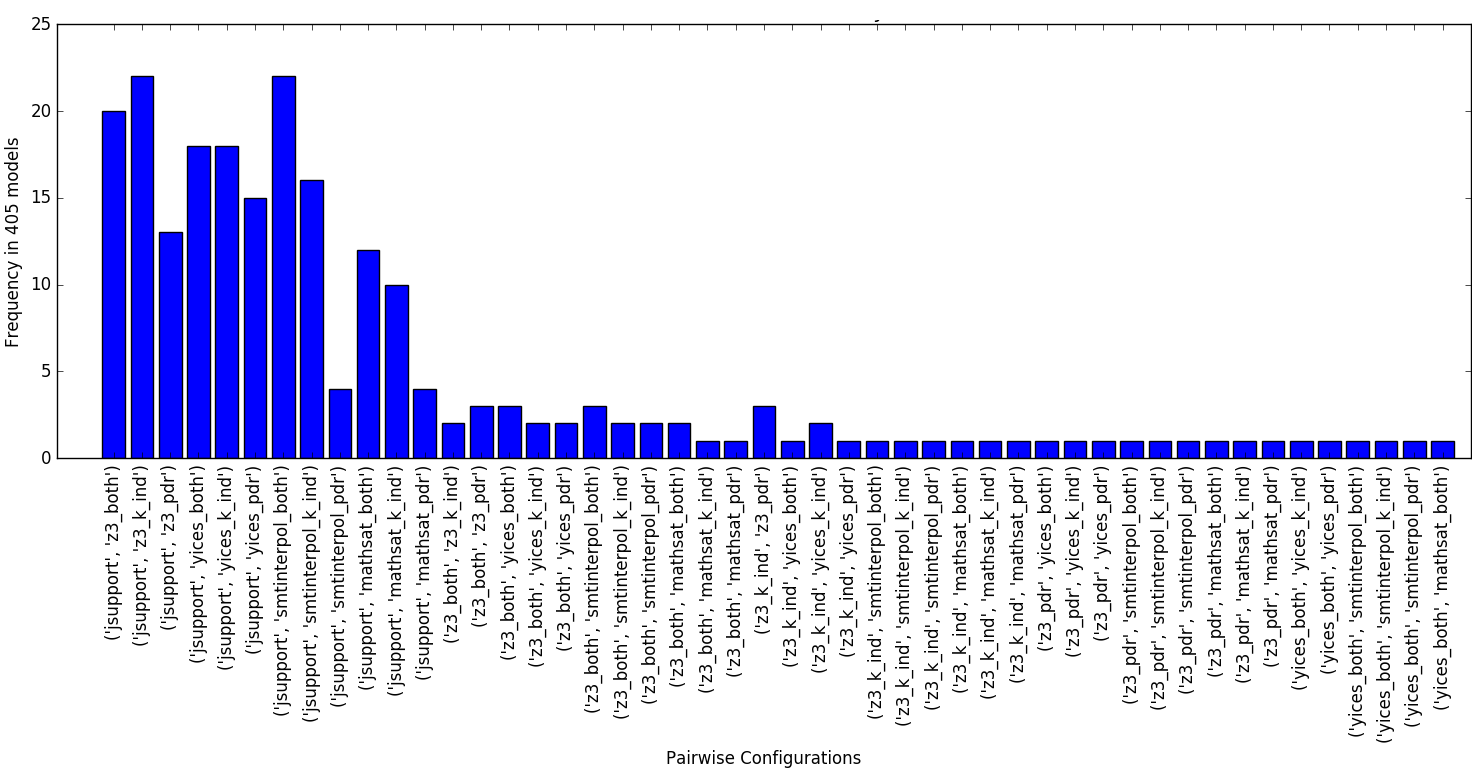
\includegraphics[width=\textwidth]{figs/max_settings_analyses.png}
%  \caption{\small{Pairwise configurations with maximum Jaccard distance}}\label{fig:maxdis}
%\end{figure}
%
%
%\begin{figure}
%  \centering
%  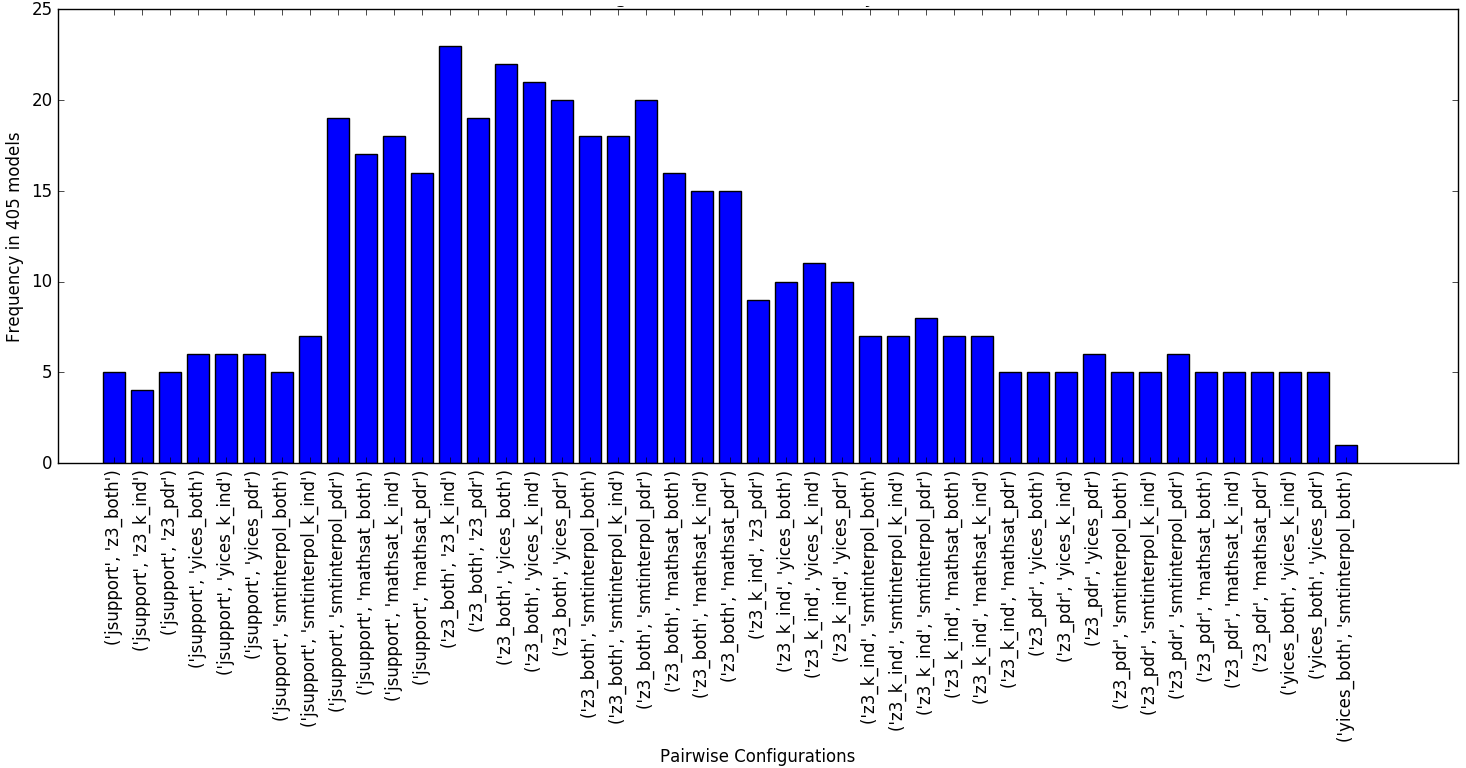
\includegraphics[width=\textwidth]{figs/min_settings_analyses.png}
%  \caption{\small{Pairwise configurations with minimum Jaccard distance}}\label{fig:mindis}
%\end{figure}

%\vspace{6pt}
%\noindent\fbox{%
%    \parbox{\textwidth}{%
%        Different solvers and proof engines have very small impact on the variety of elements in a support set of a property computed by our algorithm.
%    }%
%}
% \vspace{6pt}



%For calculations, we considered all settings where both \texttt{K-induction} and \texttt{PDR} were activated
% then in for all 405 models in everything, we collected runtime info, then calculated min/max/avg/stdev between them
% in other words, there were 4 settings to be considered: z3_both, yices_both, mathsat_both, smtinterpol_both


%\begin{figure}
%\centering
%\begin{tabular}[c]{cc}
%    \begin{subfigure}[b]{0.20\textwidth}
%      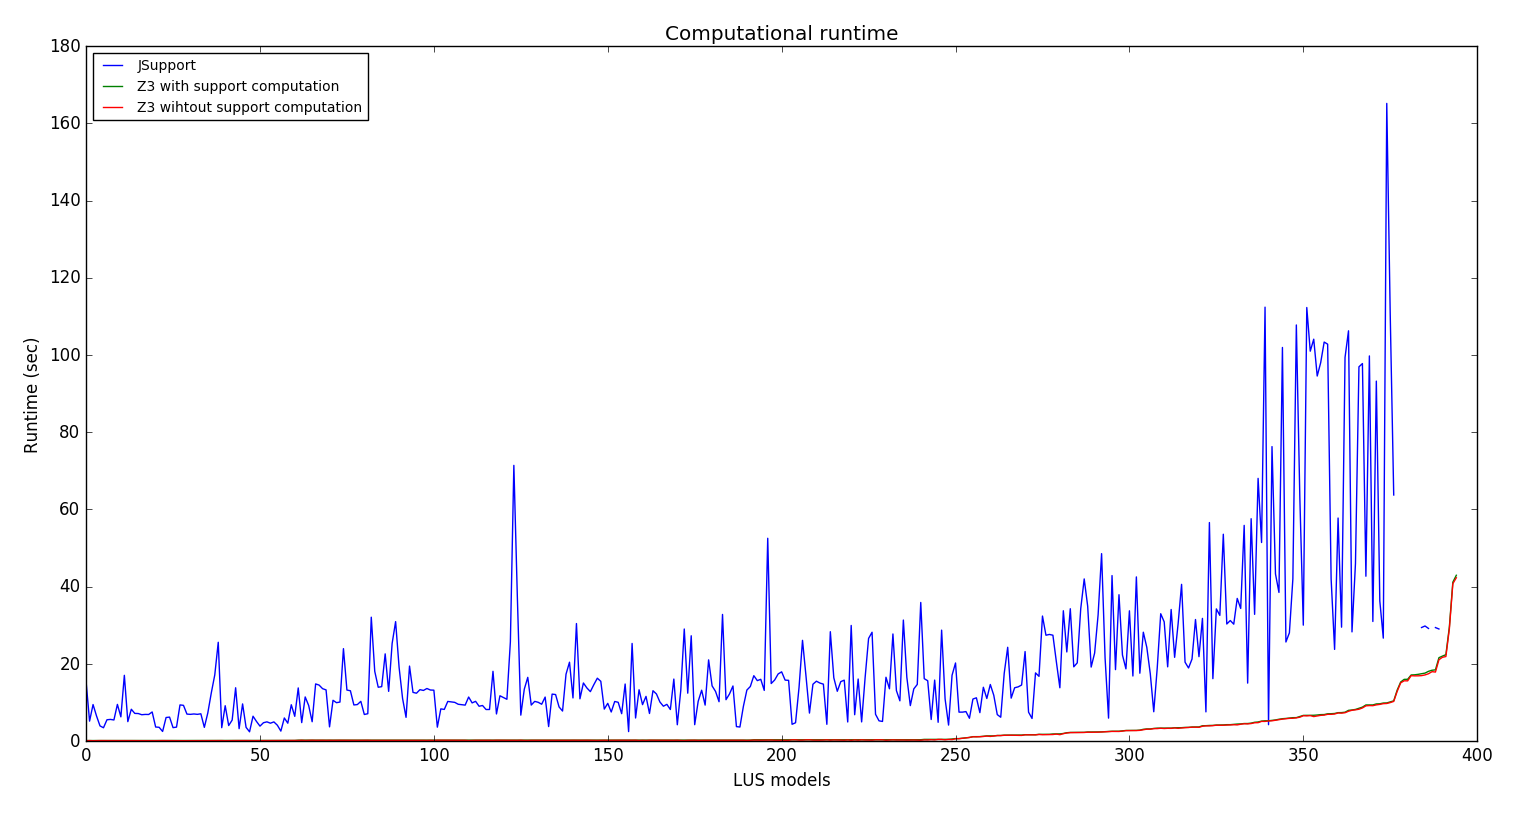
\includegraphics[width=\textwidth]{figs/figure_1.png}
%    \end{subfigure}&
%    \begin{subfigure}[b]{0.20\textwidth}
%      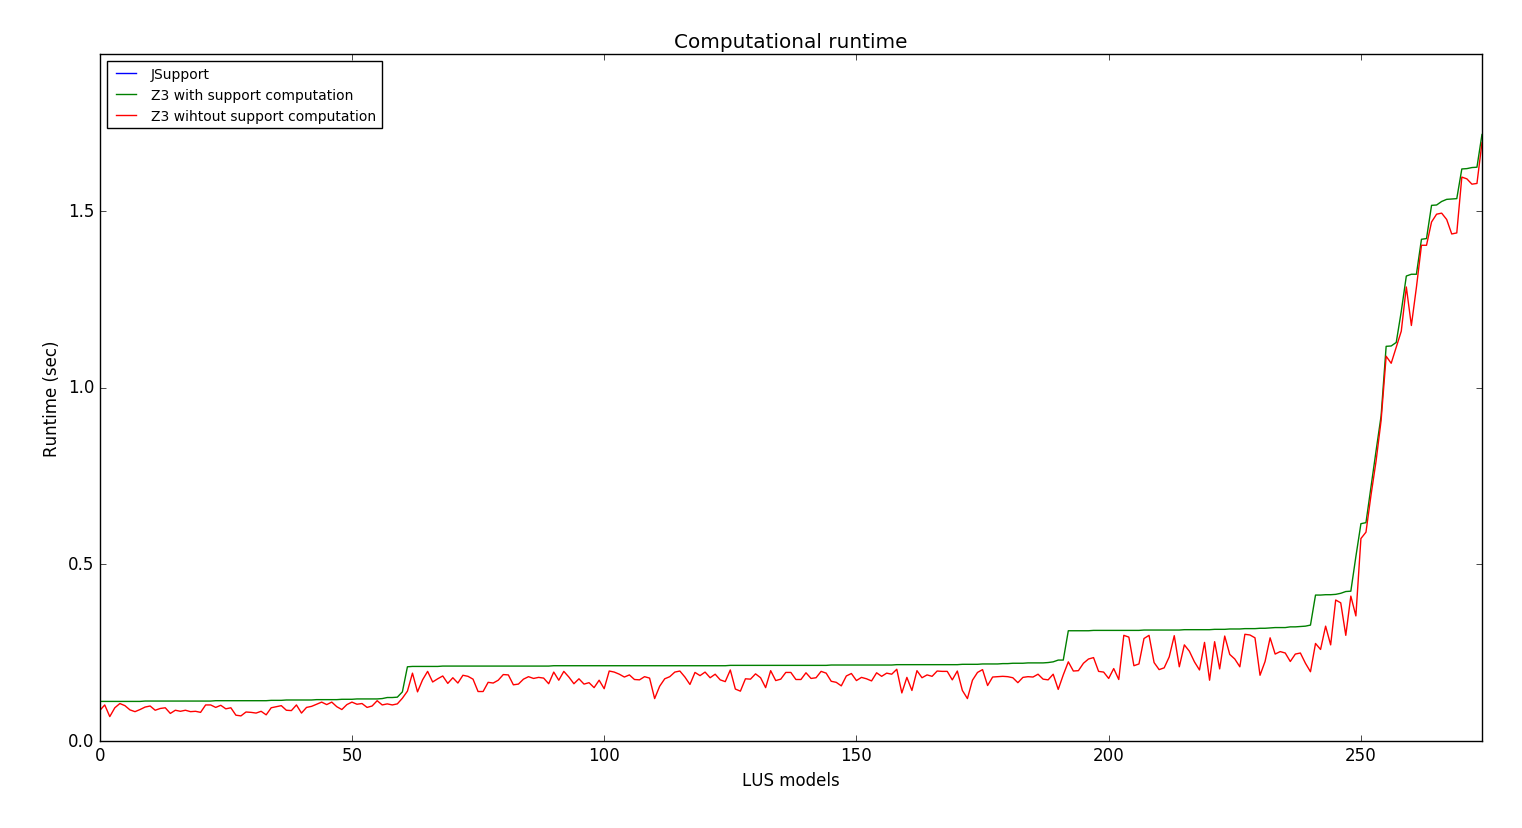
\includegraphics[width=\textwidth]{figs/figure_z3_zoom.png}
%    \end{subfigure}\\
%    \begin{subfigure}[b]{0.20\textwidth}
%      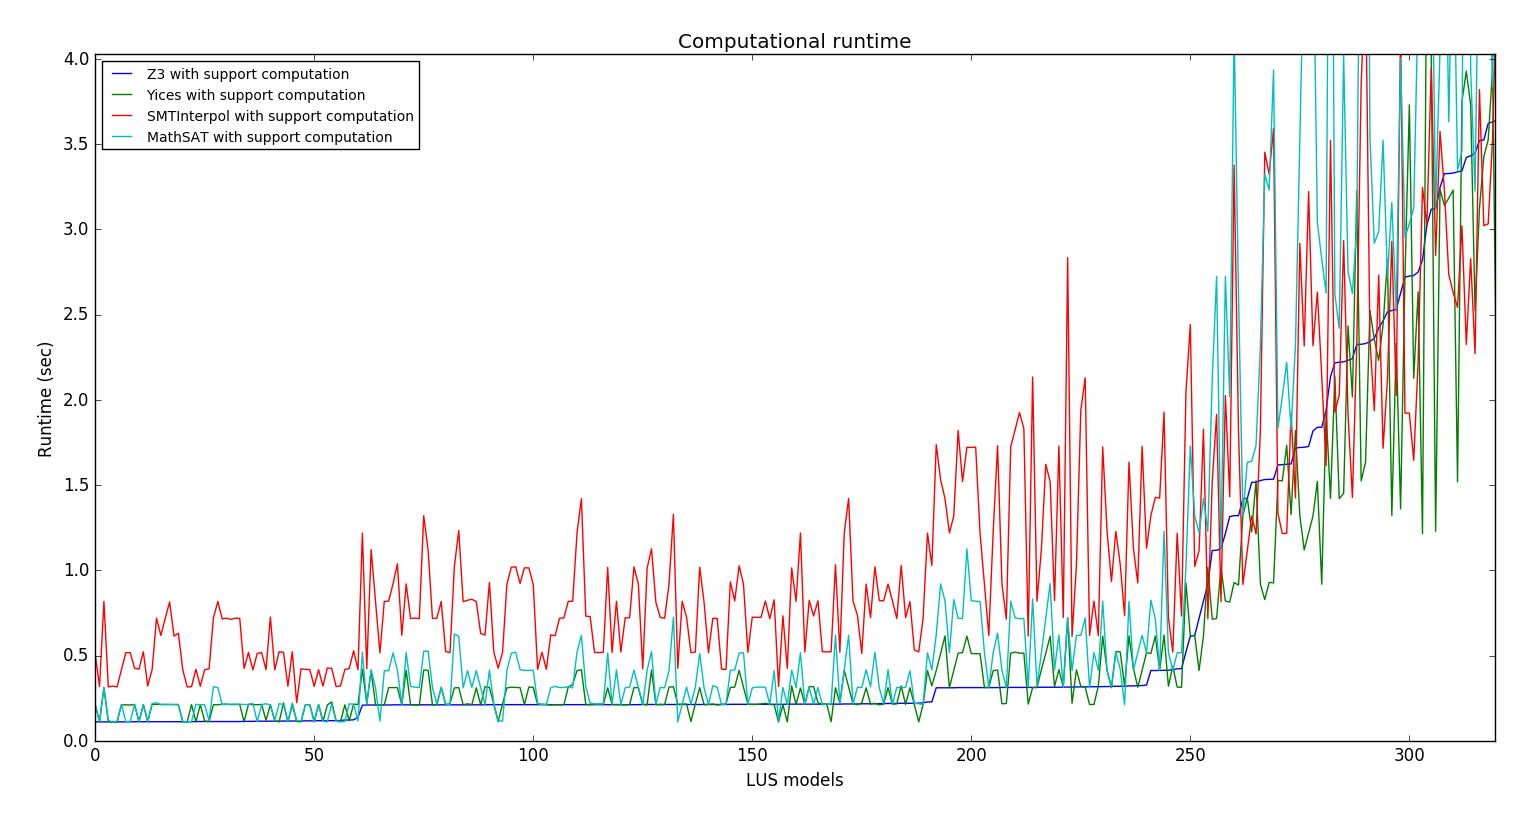
\includegraphics[width=\textwidth]{figs/solvers-support-zoom2.png}
%    \end{subfigure}&
%    \begin{subfigure}[b]{0.20\textwidth}
%      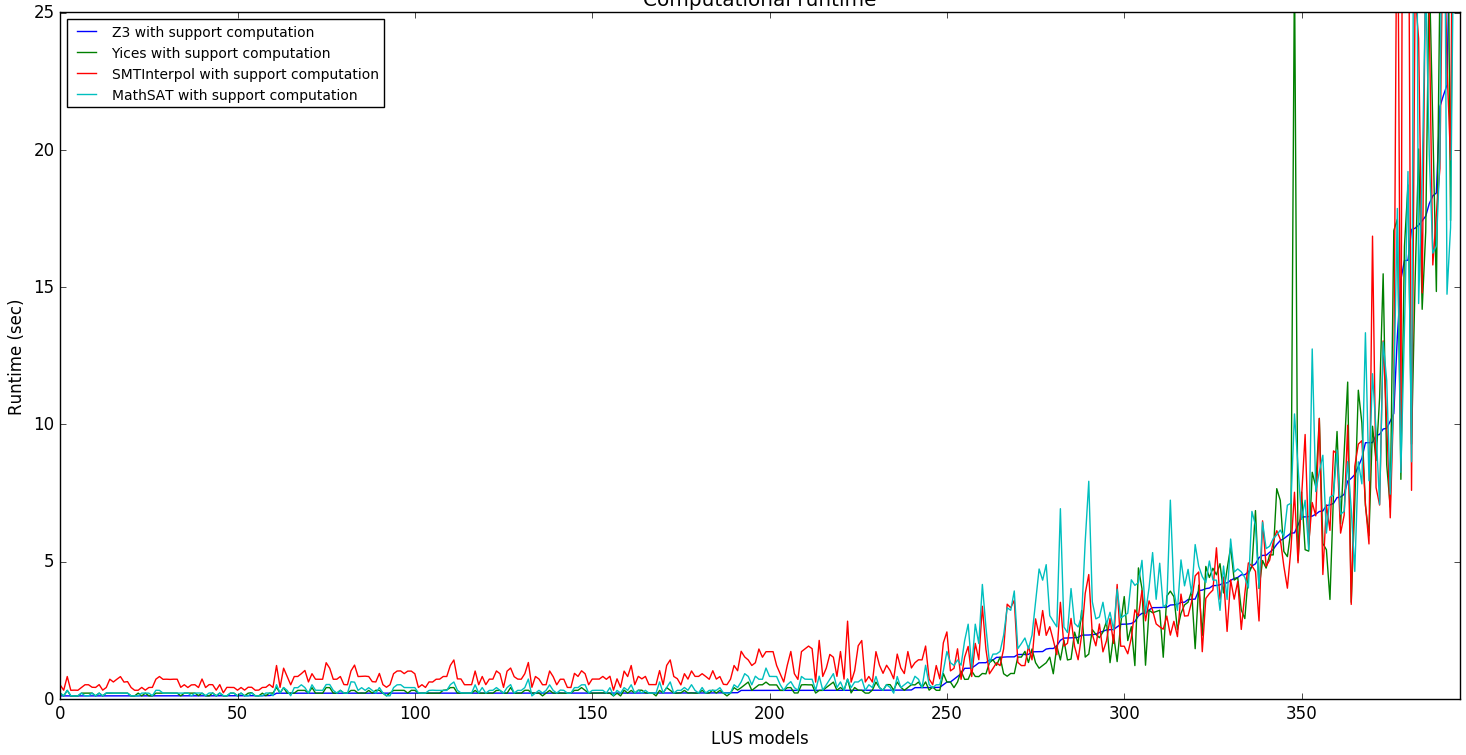
\includegraphics[width=\textwidth]{figs/solvers-support-zoom1.png}
%    \end{subfigure}
%  \end{tabular}
%\caption{\small{Runtime of support computation}}
%\label{fig:runtime}
%\end{figure}
%
%
%
%% RQ3: Is there any relationship between the size of a computed support set and
%%solvers/ proof engines?
%\textbf{RQ3:} To address this question, we analyzed the raw data with two different approaches described in the following.
%
%\textbf{(1)} We analyzed the sets of each 405 models. In each model, we looked for configurations that generated the biggest support set and ones that generated the smallest. Fig~\ref{fig:smallest} and Fig~\ref{fig:bigest} visualize the results of this analysis. For example, as you can see in Fig~\ref{fig:bigest}, \texttt{JSupport} generated biggest support sets in less than 10 models. Note that it implies there is at least one \texttt{JKind} configuration that generated the set with a smaller size.
%
%
%\begin{figure}
%  \centering
%  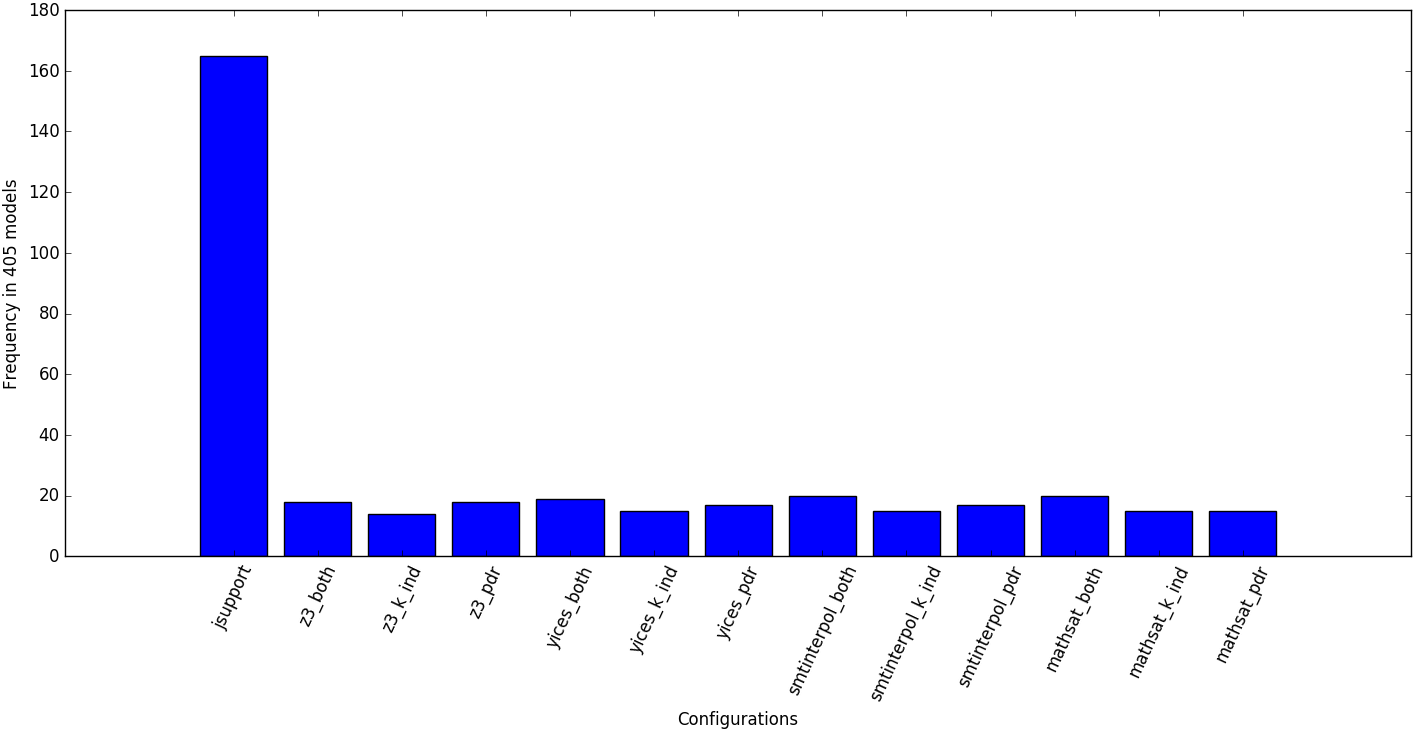
\includegraphics[width=\textwidth]{figs/small_conf.png}
%  \caption{\small{Smallest support set (in terms of size) vs configurations}}\label{fig:smallest}
%\end{figure}
%
%
%\begin{figure}
%  \centering
%  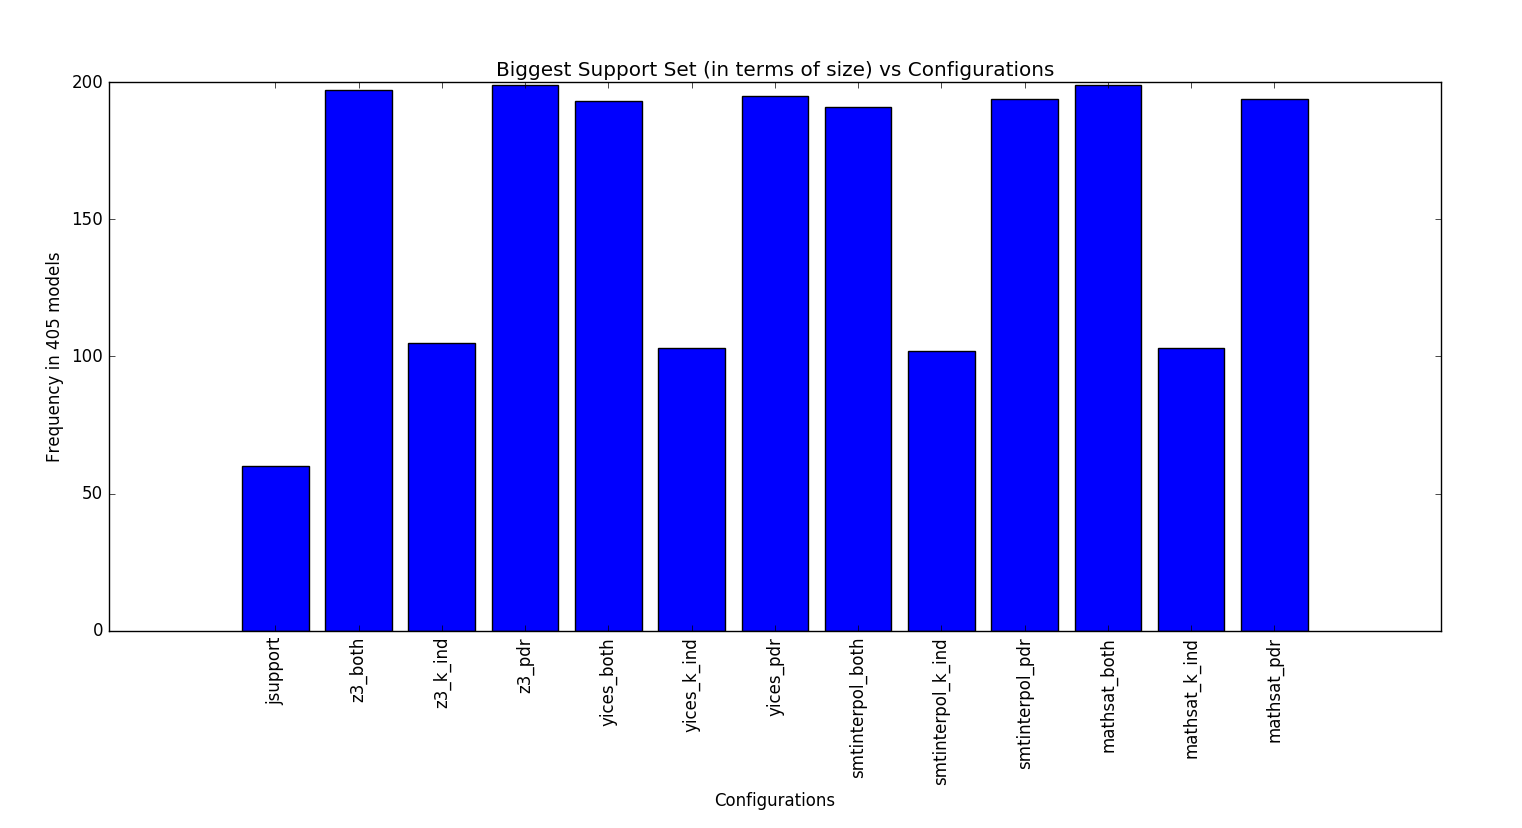
\includegraphics[width=\textwidth]{figs/big_conf.png}
%  \caption{\small{Biggest support set (in terms of size) vs configurations}}\label{fig:bigest}
%\end{figure}
%
%\vspace{6pt}
%\noindent\fbox{%
%    \parbox{\textwidth}{%
%    Solvers/ proof engines have negligible effects on the size of the support sets computed by \texttt{JKind}.
%    }%
%}
% \vspace{6pt}
%

%\textbf{RQ4:} How much {\em diversity} exists in the solutions produced by different configurations?
To measure the overall similarity among all sets, instead of a pairwise comparison, we used \emph{frequent pattern mining} \cite{han2007frequent}. To define an overall similarity among all sets of support of a given model
\footnote{Note that all models in the benchmarks are single property; hence, instead of saying a set of support of a given \emph{property}, we just refer it as the support set of the \emph{model} while explaining the experimental results.}
, we calculated a \emph{core} support set for each model in the benchmark, which can be considered as a closed frequent pattern; a core set of model $M$, denoted by $C_M$, is defined as:
\begin{definition}
  \label{def:core}
  $C_M = \bigcap_{i=1}^{13} s_{Mi},   \hspace{9pt} s_{Mi} \in S_M$
\end{definition}

Based on this notion, overall dissimilarity, denoted by $D_{J\{M\}}$, is defined as follows:

\begin{definition}
  \label{def:dis}
  $D_{J\{M\}} =  \frac{\sum_{i=1}^{12}d_J(s_{Mi}, C_M)}{12},   \hspace{9pt} s_{Mi} \in S_M$
\end{definition}

Since our goal is to measure the diversity or dissimilarity among sets computed by \texttt{ReduceSupport}, in \ref{def:dis}, we exclude the set generated by \texttt{JSupport}. In Fig~\ref{fig:jacdis}, the \emph{overall distance} line shows $D_{J\{M\}}$ per model, which can be analyzed from the following hypotheses:
\begin{itemize}
  \item H0: variety of obtained sets of support is high (average $D_{J\{M\}}$ of 0.2)
  \item H1: variety of obtained sets of support is small (average $D_{J\{M\}}$ less than 0.2)
\end{itemize}
Table~\ref{tab:variety} shows that, with an effect size of 0.79, H0 can be rejected.
\begin{table}
  \centering
  \begin{tabular}{ |c|c|c|c|c|c| }
    \hline
     min & max & mean & stdev & ES & p-value\\[0.5ex]
    \hline
    %sample size = 395
     0.0   & 0.879 & 0.096 & 0.132 & 0.79 & < 0.00001 \\[0.5ex]
    \hline
  \end{tabular}
  \caption{$D_{J\{M\}}$ among all models}
  \label{tab:variety}
\end{table}

%summarized as follows:
%\begin{itemize}
%  \item minimum $D_{J\{M\}}$ among all models: 0.0
%  \item maximum $D_{J\{M\}}$ among all models: 0.879
%  \item average $D_{J\{M\}}$ among all models: 0.096
%  \item standard deviation of $D_{J\{M\}}$ among all models: 0.132
%\end{itemize}

\vspace{6pt}
\noindent\fbox{%
    \parbox{\columnwidth}{%
    An average $D_{J\{M\}}$ of 0.096 shows that variety of support sets computed by \texttt{ReduceSupport} is very small.
    }%
}
 \vspace{6pt}

